% GENERATED BY sshrc_figures.py - edit that file, not this one.
% The document that inputs this file supplies the float, the caption and the label.
% Stream A. Committees, left to right within each year: Medieval, classics and religious studies, Economics, Business (14A, 14B, 14C), Multidisciplinary humanities, Multidisciplinary social sciences (23, 23A, 23B).
\definecolor{sshrcA}{HTML}{2A78D6}
\definecolor{sshrcB}{HTML}{EB6834}
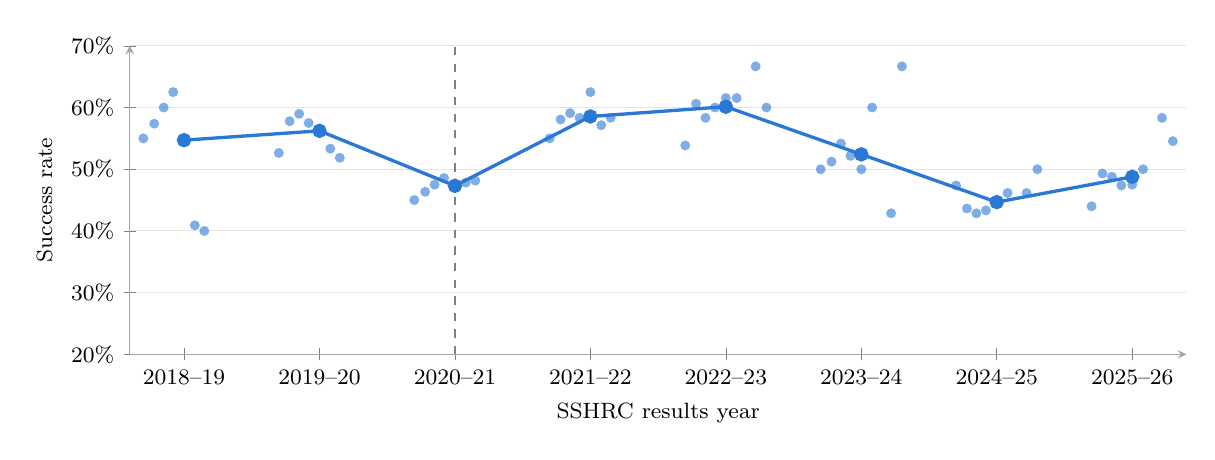
\begin{tikzpicture}
\begin{axis}[
  width=15cm, height=5.5cm,
  xmin=2017.6, xmax=2025.4, ymin=20, ymax=70,
  xtick={2018,2019,2020,2021,2022,2023,2024,2025}, xticklabels={2018--19,2019--20,2020--21,2021--22,2022--23,2023--24,2024--25,2025--26},
  axis x line=bottom, axis y line=left, axis line style={gray!70},
  ymajorgrids, grid style={gray!20},
  tick label style={font=\footnotesize}, label style={font=\footnotesize},
  xlabel={SSHRC results year}, ylabel={Success rate}, ylabel style={align=center},
  clip=false,
  ytick distance=10, yticklabel={\pgfmathprintnumber{\tick}\%},
]
\draw[gray, dashed, line width=0.7pt] (axis cs:2020,20) -- (axis cs:2020,70);
\addplot[only marks, mark=*, mark size=1.8pt, color=sshrcA,
  mark options={fill opacity=0.6, draw opacity=0}]
  coordinates {(2017.85,60.00) (2017.92,62.50) (2017.78,57.38) (2017.70,55.00) (2018.08,40.91) (2018.15,40.00) (2018.85,58.97) (2018.92,57.50) (2018.78,57.78) (2018.70,52.63) (2019.08,53.33) (2019.15,51.85) (2019.70,45.00) (2019.78,46.34) (2019.85,47.50) (2019.92,48.57) (2020.08,47.83) (2020.15,48.15) (2020.70,55.00) (2020.78,58.06) (2020.85,59.09) (2020.92,58.33) (2021.00,62.50) (2021.08,57.14) (2021.15,58.33) (2021.70,53.85) (2021.78,60.61) (2021.85,58.33) (2021.92,60.00) (2022.00,61.54) (2022.08,61.54) (2022.22,66.67) (2022.30,60.00) (2022.70,50.00) (2022.78,51.22) (2022.85,54.17) (2022.92,52.17) (2023.00,50.00) (2023.08,60.00) (2023.22,42.86) (2023.30,66.67) (2023.70,47.37) (2023.78,43.64) (2023.85,42.86) (2023.92,43.33) (2024.00,44.44) (2024.08,46.15) (2024.22,46.15) (2024.30,50.00) (2024.70,44.00) (2024.78,49.30) (2024.85,48.78) (2024.92,47.37) (2025.00,47.50) (2025.08,50.00) (2025.22,58.33) (2025.30,54.55)};
\addplot[color=sshrcA, line width=1.2pt, mark=*, mark size=2pt] coordinates {(2018.00,54.71) (2019.00,56.22) (2020.00,47.31) (2021.00,58.55) (2022.00,60.13) (2023.00,52.41) (2024.00,44.67) (2025.00,48.77)};
\end{axis}
\end{tikzpicture}
